\documentclass{tufte-handout}
% \geometry{showframe}% for debugging purposes -- displays the margins
\usepackage{wasysym}
\usepackage[utf8]{inputenc}
\usepackage[english,ngerman]{babel}

\renewcommand{\labelitemi}{$-$} % use dash for items

% Set up the images/graphics package
% \usepackage{graphicx}
% \setkeys{Gin}{width=\linewidth,totalheight=\textheight,keepaspectratio}
% \graphicspath{{graphics/}}

\title{Der Geist Mesopotamiens}
\author{Alex Schroeder}

% Set up the images/graphics package
\usepackage{graphicx}
\setkeys{Gin}{width=\linewidth,totalheight=\textheight,keepaspectratio}
\graphicspath{{graphics/}}

% The following package makes prettier tables. We're all about the
% bling!
\usepackage{booktabs}

% The units package provides nice, non-stacked fractions and better
% spacing for units.
% \usepackage{units}

% The fancyvrb package lets us customize the formatting of verbatim
% environments. We use a slightly smaller font.
% \usepackage{fancyvrb}
% \fvset{fontsize=\normalsize}

% Small sections of multiple columns
\usepackage{multicol}

\begin{document}

\maketitle% this prints the handout title, author, and date

\begin{marginfigure}
  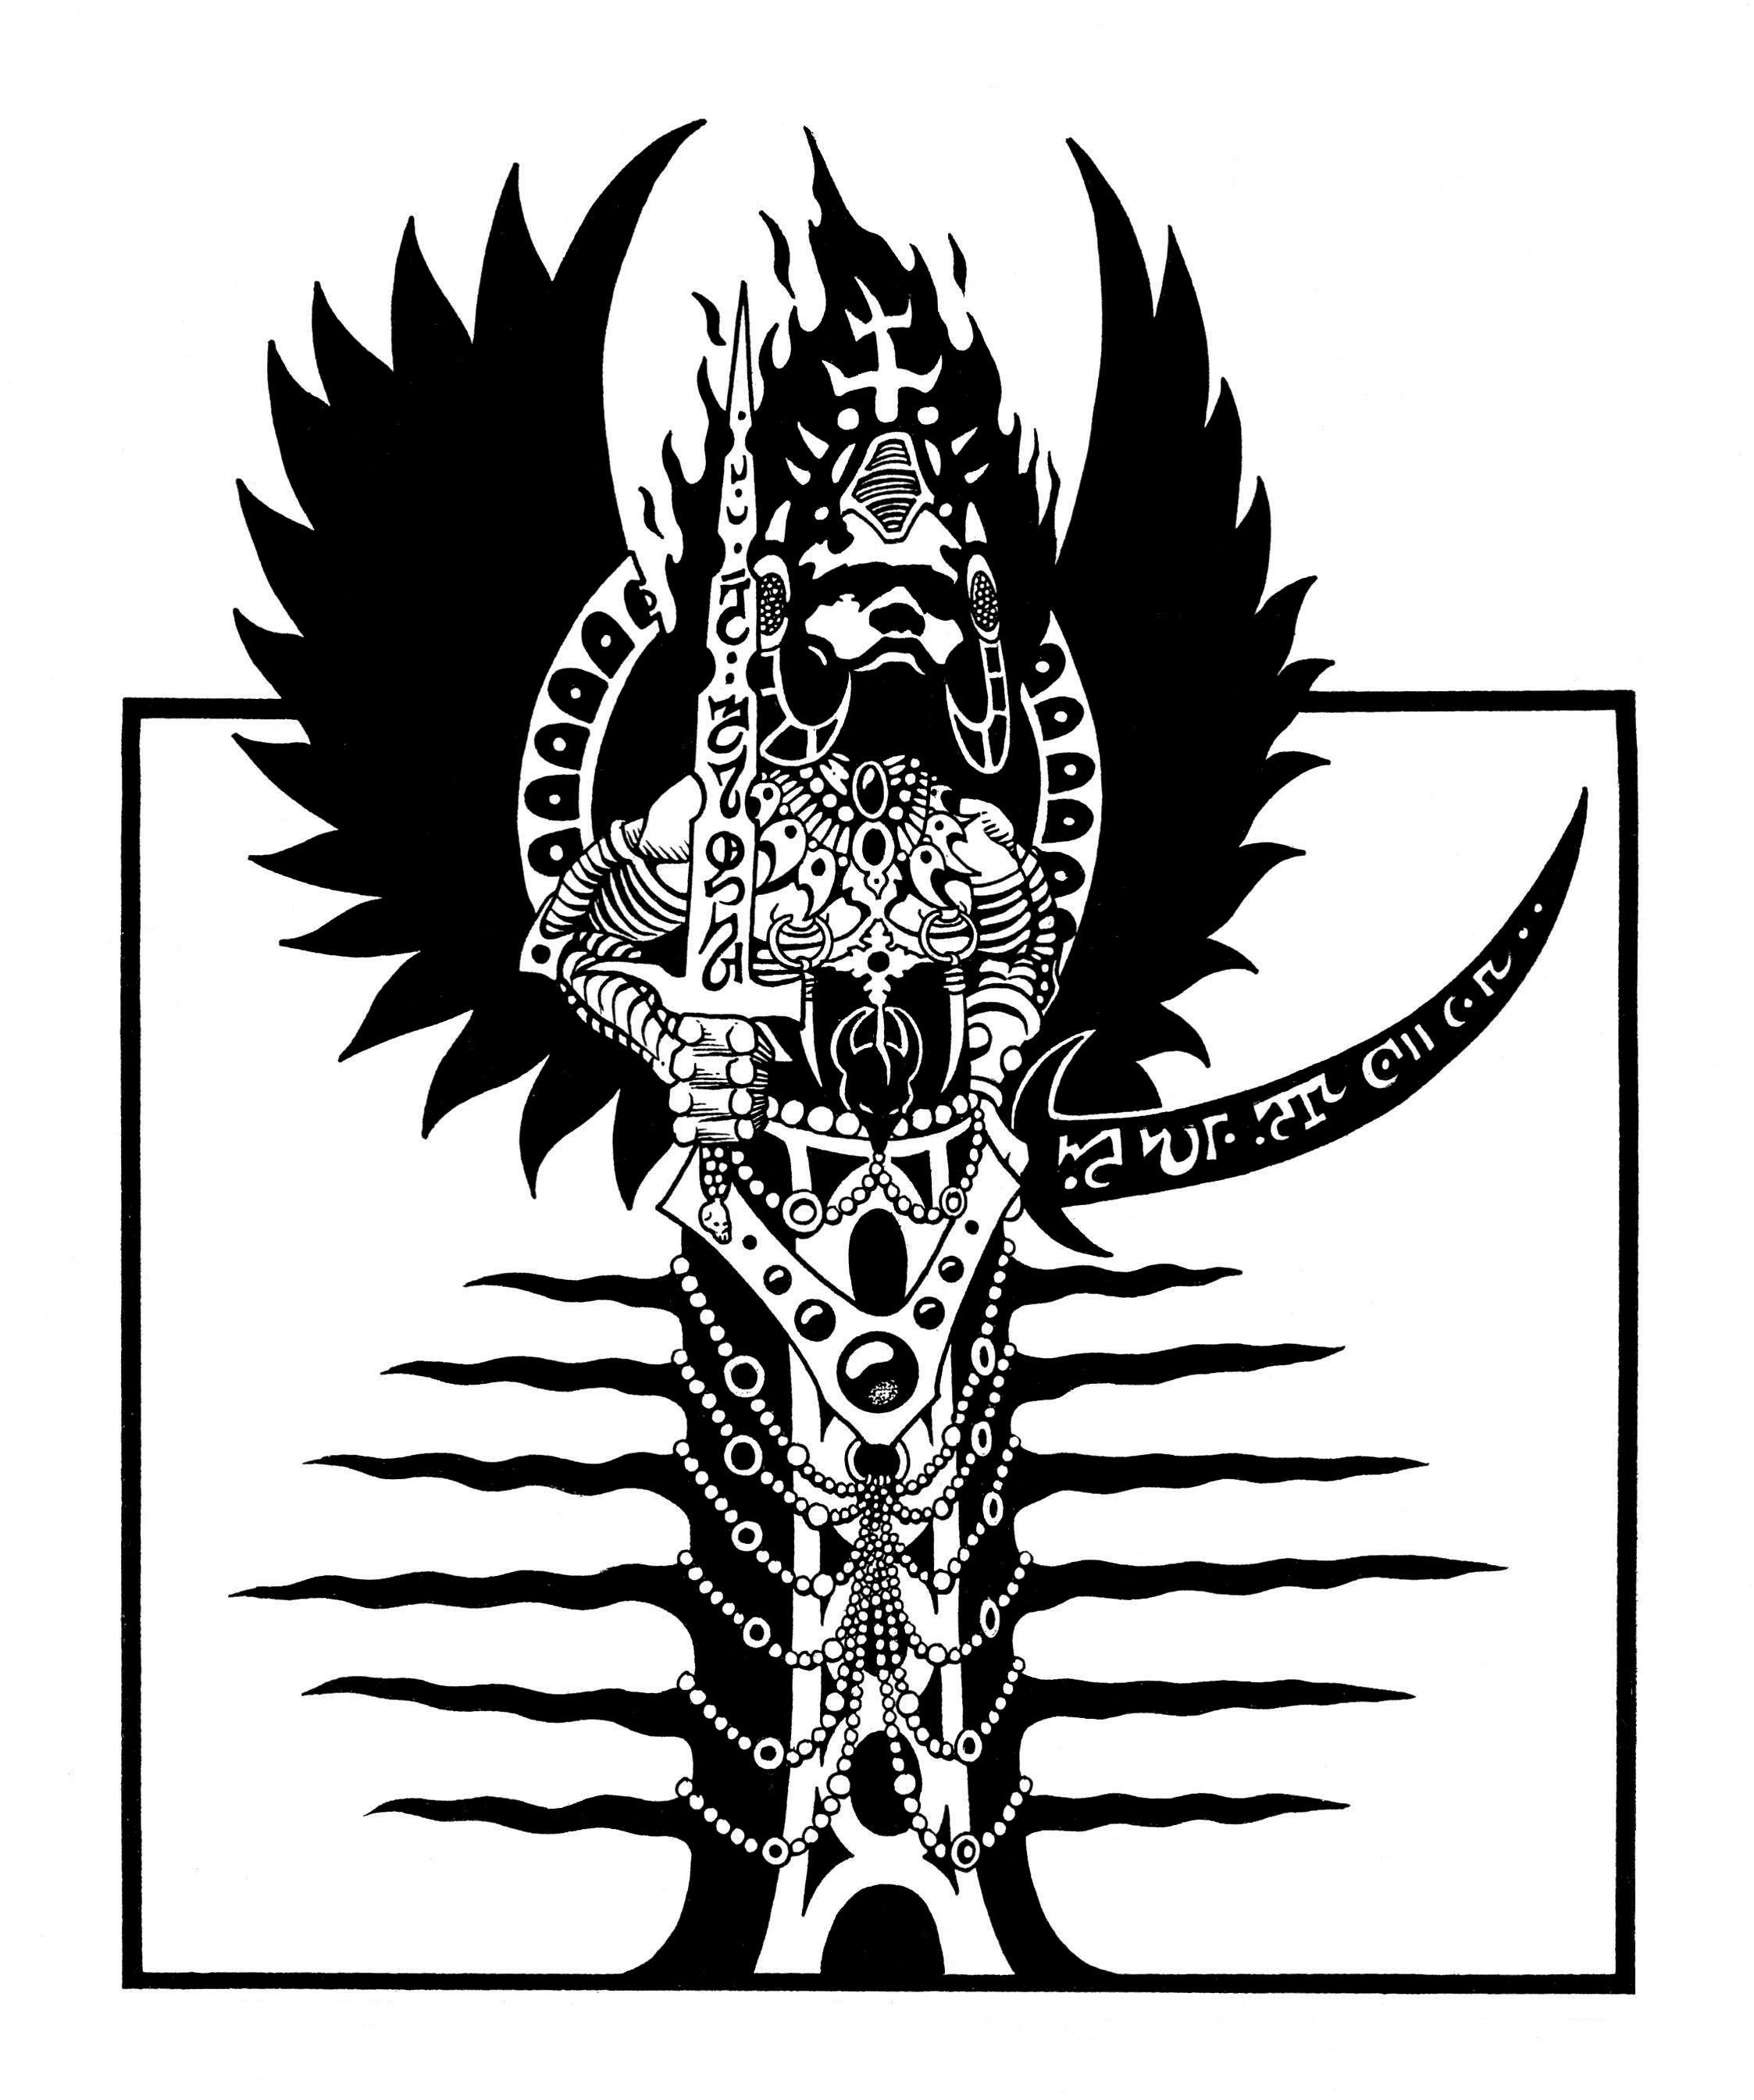
\includegraphics{pazuzu_by_tillinghast23-d37j93m.jpg}
\end{marginfigure}

\begin{abstract}
\noindent Dies sind die Regeln für unsere Mesopotamien Runde -- die
fantastische Welt der Stadtstaaten in Sparta, Athen, Ur, Babylon,
Assur, die Welt des Gilgamesch, des trojanischen Krieges, der Odyssee,
der Metamorphosen -- auf so wenig Platz wie möglich. Der
griechisch-mesopotamische Hintergrund bestimmt vor allem die Auswahl
der Fertigkeiten.
\end{abstract}


\section{Aspekte (Aspects)}

\newthought{Jeder Charakter} zwischen zwei und fünf Aspekte.
\marginnote{Herakles ist ein \textit{Sohn des Zeus},
  \textit{jähzornig} und hat \textit{übernatürliche Kraft}. Zwei
  Aspekte bleiben unbestimmt.} Diese können zusammen mit
\textit{Schicksalspunkten} verwendet werden, um Würfelergebnisse zu
verbessern. Die ersten beiden Aspekte vergibt man wie folgt:

\begin{itemize}\itemsep0pt
\item ein Charakterkonzept: Beruf, Kultur oder Persönlichkeit
\item ein Charakterfehler oder ein Beziehungsproblem
\end{itemize}

\noindent Weitere Aspekte ergeben sich idealerweise aus der
gemeinsamen Vergangenheit mit anderen Charakteren.


\section{Fertigkeiten (Skills)}

\newthought{Bei einem Test} würfelt der Spieler mit vier Fudge
Würfeln\marginnote{Herakles ist vor allem ein Ringer. Damit er nicht
  so leicht verletzt wird, wählen wir Athletik. Weil er den Bogen des
  Apollo trägt, muss er auch gut schiessen können. Da er für seine
  Keule bekannt ist, geben wir ihm die entsprechende Fertigkeit,
  obwohl die sonst kaum einer mehr verwendet.} und addiert die
passende Fertigkeit, um eine vom Spielleiter gesetzte Schwierigkeit zu
erreichen. Das Resultat kann durch den Einsatz von Aspekten und
Schicksalspunkten beeinflusst werden.

\begin{margintable}
  % we know that the margin table is 2in wide
  \begin{tabular}{cp{1.8in}}
    4 & Ringen                                                    \\
    3 & Athletik, Bogen                                           \\
    2 & Schleichen, Kurzschwert, Keule (neu)                      \\
    1 & Entschlossenheit, Muse (Leier), Streitwagen, Überleben    \\
  \end{tabular}
\end{margintable}

Wer keine Fudge Würfel hat, kann auch einen positiven und einen
negativen sechsseitigen Würfel zusammenzählen.

Die benötigte Grundausrüstung für die jeweiligen Fertigkeiten hat man
zu Spielbeginn. Wer einen Gegenstand garantiert haben will, muss
hierfür einen Trick investieren (siehe unten).

Jeder Charakter eine Fertigkeit mit Wert 4, zwei Fertigkeiten mit Wert
3, drei Fertigkeiten mit Wert 2 und vier Fertigkeiten mit Wert 1. Alle
anderen Fertigkeiten werden mit Wert 0 verwendet.

% Textblock width 6½ in
\begin{fullwidth}
\begin{tabular}{ll}
\multicolumn{2}{c}{Grundwerte}                                          \\
\midrule
Athletik         & verbessert den Zähler für Gesundheit                 \\
Entschlossenheit & verbessert den Zähler für Fassung                    \\
Mittel           & verbessert den Zähler für Vermögen                   \\
\multicolumn{2}{c}{Kämpfen}                                             \\
\midrule
Akrobatik        & Ausweichen, Bewegung auf dem Schlachtfeld            \\
Bogen            & Fernkampf                                            \\
Kurzschwert      & Nahkampf                                             \\
Reiten           & nieder reiten, verfolgen                             \\
Ringen           & auch Boxen, Schlagen                                 \\
Schild           & Verteidigen                                          \\
Schleuder        & Fernkampf                                            \\
Speer            & Nahkampf                                             \\
Speerwurf        & Fernkampf                                            \\
Streitwagen      & nieder fahren, Phalanx durchbrechen                  \\
\multicolumn{2}{c}{Zur Person}                                          \\
\midrule
Muse             & Singen, Instrumente spielen, Steinmetz, Töpfern      \\
Handeln          & Verhandeln, Geld verdienen                           \\
Rhetorik         & Leute überzeugen, Diplomatie                         \\
Überleben        & In der Wildnis überleben                             \\
Wissenschaft     & Flaschenzüge, Astronomie, Geometrie, Algebra         \\
Mystik           & Götter, Orakel, Prophezeiungen                       \\
Schleichen       & Leise sein, sich verstecken                          \\
Alchemie         & Gift, Heilmittel, Blei zu Gold, griechisches Feuer   \\
Steuermann       & Kurs finden, Strömungen erkennen                     \\
Schiffsbau       & Löcher ausbessern, neue Schiffe bauen, Mast erneuern \\
\end{tabular}
\end{fullwidth}

\bigskip
\noindent Normalerweise ist es kein Problem, wenn Spieler weitere
Fertigkeiten ins Spiel bringen.


\section{Zähler (Stress Tracks)}

\newthought{Jeder Charakter} hat drei Zähler mit je zwei Kästchen. Zu
jedem Zähler gehört eine Fertigkeit, mit der man die Anzahl Kästchen
erhöhen kann.

\marginnote[\baselineskip]{Herakles hat Athletik 4 und
  Entschlossenheit 2, deswegen hat er nicht überall zwei Kästchen:}

\begin{margintable}
  \begin{tabular}{ll}
    Gesundheit & \(\Square \Square \Square \Square\) \\
    Fassung    & \(\Square \Square \Square\)         \\
    Vermögen   & \(\Square \Square\)                 \\
  \end{tabular}
\end{margintable}

\bigskip
\begin{minipage}[t]{0.5\textwidth}
  \begin{tabular}[t]{ll}
    Zähler     & Fertigkeit       \\
    \midrule
    Gesundheit & Athletik         \\
    Fassung    & Entschlossenheit \\
    Vermögen   & Mittel           \\
  \end{tabular}
\end{minipage}
\begin{minipage}[t]{0.5\textwidth}
  \hspace{2em}
  \begin{tabular}[t]{cl}
    Wert   & Kästchen                                    \\
    \midrule
    normal & \(\Square \Square\)                         \\
    1--2   & \(\Square \Square \Square\)                 \\
    3+     & \(\Square \Square \Square \Square\)         \\
%   5      & eine weitere milde Konsequenz für den jeweiligen Zähler \\
  \end{tabular}
\end{minipage}


\section{Tricks (Stunts)}

\newthought{Jeder Charakter} hat drei Tricks.\marginnote{Herakles hat
  die folgenden drei Tricks: Einen magischen \textit{Gegenstand}, den
  Bogen des Apollo mit dem Aspekt ``Giftpfeile der Hydra'', welche
  unheilbare Wunden schlagen; die \textit{Begabung}, Schleichen im
  Kampf gegen Ahnungslose einsetzen zu können; eine
  \textit{Ersatzfähigkeit} für sich selber: so prächtig kann er
  Ringen, dass sein blosser Anblick oft stärker wirkt als jedes Wort
  -- so kann er Ringen anstelle von Rhetorik verwenden.} Ein Trick ist
einer der folgenden Vorteile:

\begin{enumerate}

\item ein \textit{Gegenstand} mit eigenem Aspekt und einer passenden
  Spezialfähigkeit; der Spielleiter kann einem diesen Gegenstand auch
  nicht wegnehmen

\item eine \textit{Begabung}: eine Fertigkeit kann auch dann
  eingesetzt werden, wenn es eigentlich nicht mehr möglich ist, oder
  ohne die Abzüge, welche Andere sonst erleiden würden

\item ein \textit{Ersatztfertigkeit} für den eigenen Charakter: eine
  bestehende Fertigkeit auf Wert 1-2 kann durch die gewählte, höhere
  Fertigkeit ersetzt werden; ohne Schicksalspunkt kann sie mit Wert 3
  eingesetzt werden; mit Schicksalspunkt kann der Wert der höheren
  Fertigkeit übernommen werden

\item eine Ersatzfertigkeit \textit{für andere}: die gewählte
  Fertigkeit kann von Begleitern eingesetzt werden; Höchstwert ist 3

\item eine \textit{Bonusfertigkeit} für andere: die gewählte Fertigkeit
  mit Mindestwert 3 kann dafür eingesetzt werden, um Begleitern einen
  +1 Bonus zu geben

\item ein weiteres \textit{Kästchen} für einen Zähler

\item eine \textit{Zählerfertigkeit}: die einem Zähler zugrunde
  liegende Fertigkeit kann durch eine andere Fertigkeit ersetzt
  werden

\end{enumerate}


\section{Schicksalspunkte (Fate Points)}

\newthought{Jeden Abend} beginnen die Charaktere mit drei
Schicksalspunkten.\marginnote{Herakles ringt gegen den nemëischen
  Löwen. Am Tisch wird entschieden, dies mit einem einfach Test
  gegeneinander zu regeln und diskutiert kurz die Konsequenzen von
  Sieg und Niederlage. Der Löwe würfelt 2 und addiert seine
  Kampfesfertigkeit von 3 zu einem Total von 5. Herakles würfelt eine
  0, addiert sein Ringen von 4 und kommt zu einem Total von 4. Der
  Spieler erzählt, dass Herakles ja \textit{übernatürliche Kraft}
  besitzt, welche er von seinem Vater geerbt hat. Er zahlt einen
  Schicksalspunkt und addiert +2 zu seinem Resultat für ein Total von
  6, und so gewinnt Herakles dank der Macht des Schicksals. Es bleiben
  ihm zwei Schicksalspunkte für den Rest des Abends.} Diese setzt man
nach dem Würfeln ein: Man erzählt, warum ein Aspekt die Situation
beeinflusst und wenn alle einverstanden sind, \textbf{addiert man +2}
auf den Wurf oder \textbf{würfelt noch mal}.

Wer dem Spielleiter einen Vorschlag zum eigenen Nachteil vorschlägt,
erhält einen Schicksalspunkt, wenn der Spielleiter darauf eingeht.

Wer einen Vorschlag des Spielleiters zum eigenen Nachteil annimmt,
erhält einen Schicksalspunkt; anderenfalls muss ein Schicksalspunkt
gezahlt werden. Im Kampf nimmt dies meistens die Form von ``setzen
eine Runde aus und nimm dafür einen Schicksalspunkt.''


\section{Kampfrunden}

\marginnote{Herakles ringt mit dem kretischen Stier. Dieser verwüstet
  die ganze Insel: Hörner 4, Trampeln 3, Gesundheit \(\Square
  \Square\). Es gibt den lokalen Aspekt \textit{Die Sonne brennt vom
    Himmel}. Herakles hat Ringen 4, Athletik 3 und zwei
  Schicksalspunkte. Der dritte Schicksalspunkt wurde im letzten
  Beispiel schon gebraucht.

\textbf{Erste Runde}: Herakles würfelt 0, addiert Ringen 4, gibt 4.
Der Stier würfelt -1, addiert Hörner 4, gibt 3. Herakles entscheidet
sich, die brennende Sonne zu seinem Vorteil zu verwenden und zahlt
einen Schicksalspunkt für +2, gibt 6. Die Differenz ist nun 3
zugunsten von Herakles. Die Differenz führt zu einem zusätzlichen,
temporären Aspekt: Der Stier ist ``verwirrt''. Der Stier nimmt eine
milde (-2) Konsequenz und endet \textit{im Würgegriff}; zudem ist
seine Gesundheit \(\XBox \Square\). Der Stier greift zurück an und
würfelt 1, addiert Hörner 4, gibt 5. Herakles würfelt -2. Der Spieler
meint, dass Herakles der \textit{Sohn des Zeus} ist, und seines Vaters
Segen ihm hilft. Er zahlt den letzten Schicksalspunkt und würfelt -3!
Pech gehabt. Der Spieler beschliesst, den freien Aspekt ``verwirrt''
zu verwenden und würfelt -1, addiert Ringen 4, und verwendet den
zweiten freien Aspekt ``im Würgegriff'' für +2, gibt 5. Gleichstand!
Ein temporärer Aspekt ist für den angreifenden Stier enstanden:
Herakles ist \emph{niedergeworfen}.

\textbf{Zweite Runde}: Herakles greift an und würfelt 0, addiert
Ringen 4, gibt 4. Der Stier würfelt -3, addiert Hörner 4 und verwendet
den Aspekt \emph{niedergeworfen} für +2, gibt 3. Die Differenz ist 1
zugunsten von Herakles. Da die Gesundheit des Stiers schon \(\XBox
\Square\) ist, muss trotzdem das zweite Kästchen genommen werden:
\(\XBox \XBox\). Der Stier greift zurück an und würfelt -1, addiert
Hörner 4, gibt 3. Herkules würfelt 0, addiert Ringen 4, gibt 4. Der
Angriff schlägt fehl.

\textbf{Dritte Runde}: Herakles greift an und würfelt 1, addiert
Ringen 4, gibt 5. Der Stier würfelt 0, addiert Hörner 4, gibt 4. Die
Kästchen sind voll, die milde Konsequenz ist schon genommen: Es muss
eine mittlere (-4) Konsequenz sein: \textit{Die Hörner sind
  abgebrochen}. Der Stier gibt auf und bietet die Gefangenschaft an.
Herakles akzeptiert.}

\newthought{In jeder Runde} kann man sich um eine Zone auf der Karte
bewegen (falls es eine Karte gibt) \textit{und} eine der folgenden
Aktionen durchführen:

\begin{enumerate}
\item \textit{Überwinden}: ein Hindernis mit einer Fertigkeit
  überwinden (z.\,B.~eine grössere Distanz mit Akrobatik überwinden)
\item \textit{Vorteil schaffen}: ein Aspekt wird eingeführt, der
  von der eigenen Seite ein Mal frei zu verwenden ist; 
\item \textit{Angreifen} (siehe unten)
\end{enumerate}

\noindent In allen Fällen wird die Schwierigkeit entweder vom
Spielleiter festgelegt oder es gibt einen Gegner, der sich der Aktion
widersetzt und hierfür eine entsprechende Fertigkeit verwendet.

Gelingt die Aktion mit einer Differenz von mindestens drei, so
entsteht ein neuer, temporärer Aspekt, den man ein Mal frei verwenden
darf. Bei Gleichstand entsteht auch ein neuer, temporärer Aspekt, den
der Handelnde oder der Angreifer ein Mal frei verwenden darf.


\subsection{Angreifen}

Um Anzugreifen, würfelt man die Fudge Würfel und addiert die passende
Fertigkeit und zieht die Zonendifferenz ab, wenn man sich nicht in der
gleichen Zone befindet. Um Abzuwehren, würfelt man die Fudge Würfel
und addiert eine passende Fertigkeit. Der Verteidigungswurf gilt gegen
alle Angriffe dieser Runde.

Ist die Differenz zum Vorteil des Angreifers, ist dieser Wert auf dem
entsprechenden Zähler einzutragen. Ist das entsprechende Kästchen
voll, muss ein höheres Kästchen genommen werden. Gibt es kein freies
Kästchen mehr, müssen Konsequenzen genommen werden, um dies zu
kompensieren.

Man kann drei Konsequenzen nehmen: Die milde Konsequenz ist zwei
Kästchen wert, die mittlere Konsequenz ist vier Kästchen wert und die
schwere Konsequenz ist sechs Kästchen wert. Konsequenzen sind Aspekte,
welche für die Gegenseite ein mal frei zu verwenden sind. Kann der
Schaden nicht mehr kompensiert werden, scheidet man aus. Man kann dem
Gegner auch jederzeit eine Konzession anbieten und aufgeben.

Nach einer kurzen Verschnaufpause werden die Kästchen aller Zähler
wieder frei. Nur die Konsequenzen bleiben.

\clearpage


\section{Ende des Spielabends}

\marginnote{Herakles hat den Stier gebändigt. Er gibt sich den Aspekt
  \textit{Tierbändiger} und tauscht Mystik mit Muse aus, weil er sich
  seinem göttlichen Erbe näher fühlt und sowieso nie die Leier rührt.
  Er muss keinen Aspekt streichen, weil er ja noch nicht alle fünf
  gewählt hat.}

\newthought{Am Ende des Abends} darf man

\begin{itemize}
\item zwei nebeneinander liegende Fertigkeiten tauschen
\item ein Aspekt austauschen
\item eine milde Konsequenz streichen
\item eine mittlere Konsequenz streichen, die man an einem \textit{früheren}
  Spielabend erlitten hat
\item eine schwere Konsequenz streichen, die man an einem
  \textit{früheren} Spielabend erlitten hat, falls man für diesen
  Zähler dieses mal kein einziges Kästchen verloren hat
\end{itemize}

\vspace{3cm}

\begin{fullwidth}
\centering

\includegraphics[height=10cm]{pazuzu_dagger_by_tillinghast23-d392ool.jpg}
\end{fullwidth}

\clearpage


\section{Lizenz: Open Game License Version 1.0a}

\fontsize{7.5pt}{8pt}\selectfont

\begin{fullwidth}
The following text is the property of Wizards of the Coast, Inc. and
is Copyright 2000 Wizards of the Coast, Inc (``Wizards''). All Rights
Reserved.

\begin{enumerate}

\item Definitions: (a) ``Contributors'' means the copyright and/or
  trademark owners who have contributed Open Game Content; (b)
  ``Derivative Material'' means copyrighted material including
  derivative works and translations (including into other computer
  languages), potation, modification, correction, addition, extension,
  upgrade, improvement, compilation, abridgment or other form in which
  an existing work may be recast, transformed or adapted; (c)
  ``Distribute'' means to reproduce, license, rent, lease, sell,
  broadcast, publicly display, transmit or otherwise distribute; (d)
  ``Open Game Content'' means the game mechanic and includes the
  methods, procedures, processes and routines to the extent such
  content does not embody the Product Identity and is an enhancement
  over the prior art and any additional content clearly identified as
  Open Game Content by the Contributor, and means any work covered by
  this License, including translations and derivative works under
  copyright law, but specifically excludes Product Identity. (e)
  ``Product Identity'' means product and product line names, logos and
  identifying marks including trade dress; artifacts; creatures
  characters; stories, storylines, plots, thematic elements, dialogue,
  incidents, language, artwork, symbols, designs, depictions,
  likenesses, formats, poses, concepts, themes and graphic,
  photographic and other visual or audio representations; names and
  descriptions of characters, spells, enchantments, personalities,
  teams, personas, likenesses and special abilities; places,
  locations, environments, creatures, equipment, magical or
  supernatural abilities or effects, logos, symbols, or graphic
  designs; and any other trademark or registered trademark clearly
  identified as Product identity by the owner of the Product Identity,
  and which specifically excludes the Open Game Content; (f)
  ``Trademark'' means the logos, names, mark, sign, motto, designs
  that are used by a Contributor to identify itself or its products or
  the associated products contributed to the Open Game License by the
  Contributor (g) ``Use'', ``Used'' or ``Using'' means to use,
  Distribute, copy, edit, format, modify, translate and otherwise
  create Derivative Material of Open Game Content. (h) ``You'' or
  ``Your'' means the licensee in terms of this agreement.

\item The License: This License applies to any Open Game Content that
  contains a notice indicating that the Open Game Content may only be
  Used under and in terms of this License. You must affix such a
  notice to any Open Game Content that you Use. No terms may be added
  to or subtracted from this License except as described by the
  License itself. No other terms or conditions may be applied to any
  Open Game Content distributed using this License.

\item Offer and Acceptance: By Using the Open Game Content You
  indicate Your acceptance of the terms of this License.

\item Grant and Consideration: In consideration for agreeing to use
  this License, the Contributors grant You a perpetual, worldwide,
  royalty- free, non-exclusive license with the exact terms of this
  License to Use, the Open Game Content.

\item Representation of Authority to Contribute: If You are
  contributing original material as Open Game Content, You represent
  that Your Contributions are Your original creation and/or You have
  sufficient rights to grant the rights conveyed by this License.

\item Notice of License Copyright: You must update the COPYRIGHT
  NOTICE portion of this License to include the exact text of the
  COPYRIGHT NOTICE of any Open Game Content You are copying, modifying
  or distributing, and You must add the title, the copy- right date,
  and the copyright holder's name to the COPYRIGHT NOTICE of any
  original Open Game Content you Distribute.

\item Use of Product Identity: You agree not to Use any Product
  Identity, including as an indication as to compatibility, except as
  expressly licensed in another, independent Agreement with the owner
  of each element of that Product Identity. You agree not to indicate
  compatibility or co-adaptability with any Trademark or Registered
  Trademark in conjunction with a work containing Open Game Content
  except as expressly licensed in another, independent Agreement with
  the owner of such Trademark or Registered Trademark. The use of any
  Product Identity in Open Game Content does not constitute a
  challenge to the ownership of that Product Identity. The owner of
  any Product Identity used in Open Game Content shall retain all
  rights, title and interest in and to that Product Identity.

\item Identification: If you distribute Open Game Content You must
  clearly indicate which portions of the work that you are distrib-
  uting are Open Game Content.

\item Updating the License: Wizards or its designated Agents may
  publish updated versions of this License. You may use any autho-
  rized version of this License to copy, modify and distribute any
  Open Game Content originally distributed under any version of this
  License.

\item Copy of this License: You MUST include a copy of this License
  with every copy of the Open Game Content You Distribute.

\item Use of Contributor Credits: You may not market or advertise the
  Open Game Content using the name of any Contributor unless You have
  written permission from the Contributor to do so.

\item Inability to Comply: If it is impossible for You to comply with
  any of the terms of this License with respect to some or all of the
  Open Game Content due to statute, judicial order, or governmental
  regulation then You may not Use any Open Game Material so affected.

\item Termination: This License will terminate automatically if You
  fail to comply with all terms herein and fail to cure such breach
  within 30 days of becoming aware of the breach. All sublicenses
  shall survive the termination of this License.

\item Reformation: If any provision of this License is held to be
  unenforceable, such provision shall be reformed only to the extent
  necessary to make it enforceable.

\item COPYRIGHT NOTICE\newline Open Game License v 1.0 © 2000, Wizards
  of the Coast, Inc.\newline \href{http://www.fudgerpg.com/}{Fudge
    System} 1995 version © 1992-1995 by Steffan O'Sullivan, © 2005 by
  Grey Ghost Press, Inc.; Author Steffan O'Sullivan.\newline
  \href{http://www.faterpg.com/}{\textsf{FATE}} (Fantastic Adventures
  in Tabletop Entertainment) © 2003 by Evil Hat Productions LLC;
  Authors Robert Donoghue and Fred Hicks.\newline
  \href{http://www.crackmonkey.org/\%7Enick/loyhargil/fate3/fate3.html}{Spirit
    of the Century} © 2006, Evil Hat Productions LLC. Authors Robert
  Donoghue, Fred Hicks, and Leonard Balsera.\newline
  \href{http://www.vsca.ca/Diaspora/diaspora-srd.html}{Diaspora} ©
  VSCA Publishing. Authors Brad Murray, C.W. Marshall, Tim Dyke and
  Byron Kerr.\newline
  \href{http://campaignwiki.org/wiki/MontagInZürich/Der_Geist_Mesopotamiens}{Der
    Geist Mesopotamiens} © 2010--2013 by Alex Schröder.

\end{enumerate}

\noindent For purposes of this license, the two images by Erik York
are Product Identity. You can find more of his art and contact him at
\href{http://tillinghast23.deviantart.com/}{tillinghast23.deviantart.com}.
The game text without the license itself is Open Game Content.

\end{fullwidth}

\nobibliography{}
\end{document}
